\documentclass[aspectratio=169]{beamer}
\usetheme{metropolis}

%\usepackage{pgfpages}
%\setbeameroption{show notes}
%\setbeameroption{show notes on second screen=right}

\usepackage[english]{babel}
\usepackage[utf8]{inputenc}
\usepackage{amsmath, amssymb, amsthm, amsfonts}
\usepackage{multimedia}
\usepackage{graphics}
\usepackage{hyperref}

\usepackage{caption}
\usepackage{subcaption}

\title{Generelle Statistiske Metoder}
\author{Erik Rybakken}

\begin{document}

\frame{\titlepage}

\begin{frame}
  \frametitle{Framingham Datasett}
  \begin{itemize}
    \item Studie av 4434 pasienter, med fokus på hjerteproblemer.
    \pause
    \item Hver pasient ble undersøkt tre ganger, med 6 års mellomrom.
  \end{itemize}

  \pause

  To mulige problemstillinger:
  \begin{enumerate}
    \item Hvilke prediktorer påvirker blodtrykket?
    \pause
    \item Kan vi forutsi hvor lenge en pasient har igjen å leve basert på dataene som ble gjort i første sjekk?
  \end{enumerate}
  \pause
  Detaljer om analysen:
  \begin{enumerate}
    \item Kun pasientene fra den første sjekken ble brukt i analysen
    \pause
    \item Paientene med minst én ukjent verdi ble fjernet fra analysen
    \pause
    \item Dette ble i alt 3885 pasienter
  \end{enumerate}
\end{frame}

\begin{frame}
  \frametitle{Lineær regresjon}
  Vi antar en lineær modell:
  \begin{equation}
    Y = X \beta + \epsilon
  \end{equation}
  \pause
  der
  \begin{itemize}
    \item \(Y\) er responsen
    \item \(X\) er prediktorene
    \item \(\beta\) er en vektor med koeffisienter
    \item \(\epsilon\) er en normalfordelt variabel med forventningsverdi 0
  \end{itemize}
  \pause
  I vårt tilfelle er \(Y\) blodtrykket, mens \(X\) består av prediktorene kjønn (mann/kvinne), alder,
  antall sigaretter røyket per dag, BMI, glukosenivå, utdanningsnivå og kolesterolnivå.
\end{frame}

\begin{frame}
  \frametitle{Minstre kvadraters metode}

  Vi har en \(n\times p\)-matrise \(\textbf{X}\) bestående av n observasjoner av p prediktorer, og en \(n\times 1\)-matrise \(\textbf{Y}\) bestående av de korresponderene responsvariablene. Vi vil fra nå av anta at de observerte prediktorene og responsene er normalisert til å ha gjennomsnitt 0 og varians 1.

  \pause

  Minstre kvadraters metode estimerer koeffisientene \(\beta\) ved å minimere RSS (residual sum of squares):

  \begin{equation}
    (\textbf{Y} - \textbf{X}\beta)^T (\textbf{Y} - \textbf{X}\beta)
  \end{equation}
\end{frame}

\begin{frame}
  \frametitle{Tre modifiseringer av minste kvadraters metode}
  \begin{itemize}
    \item Beste delmengde-utvalg velger ut en delmengde av prediktorene og utfører minstre kvadrater på denne.
    \pause
  \item Lasso-regresjon krymper absoluttverdien til koeffisientene \(\beta\).
    \pause
    \item Prinsipalkomponent-regresjon projiserer først prediktorene til et lavere-dimensjonalt underrom og utfører deretter minstre kvadrater.
  \end{itemize}
\end{frame}

\begin{frame}
  \frametitle{Beste delmengde-utvalg}
  Gitt en delmengde \(S \subset \{1,\dots,p\}\) kan vi danne matrisen \(\textbf{X}_S = (\textbf{X}_{i_1}|\textbf{X}_{i_2}|\dots |\textbf{X}_{i_k})_{i_* \in S}\).
  Vi kan så utføre minst kvadrater på \(\textbf{X}_S\).
  \pause
  For en gitt \(0 \leq k \leq p\) utfører vi minste kvadrater på den \(\textbf{X}_S\) med \(|S| = k\) som gir lavest RSS.
\end{frame}

\begin{frame}
  \frametitle{Beste delmengde-utvalg}
  \begin{center}
    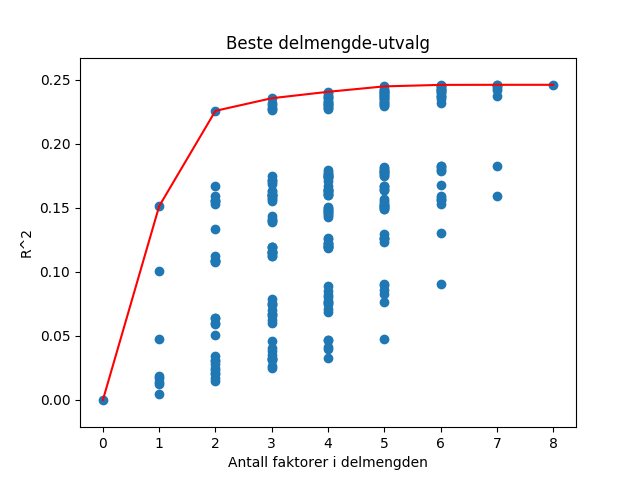
\includegraphics[height=0.8\textheight]{best_subset.png}
  \end{center}
\end{frame}

\begin{frame}
  \frametitle{Lasso-regresjon}
  Lasso-regresjon finner koeffisientene \(\beta\) som minimerer uttrykket
  \begin{equation}
    (\textbf{Y} - \textbf{X}\beta)(\textbf{Y} - \textbf{X}\beta)^T + \lambda \sum_{i=1}^p |\beta_i|
  \end{equation}
  der \(\lambda\) er en parameter som bestemmer hvor mye koeffisientene skal krympes.
  
  \pause
  Dette er ekvivalent med å minimere uttrykket
  \begin{equation}
    (\textbf{Y} - \textbf{X}\beta)^T (\textbf{Y} - \textbf{X}\beta)
  \end{equation}
  der vi krever at \(\sum_{i=1}^p |\beta_i| \leq t\).
\end{frame}

\begin{frame}
  \frametitle{Lasso-regresjon}
  \begin{center}
    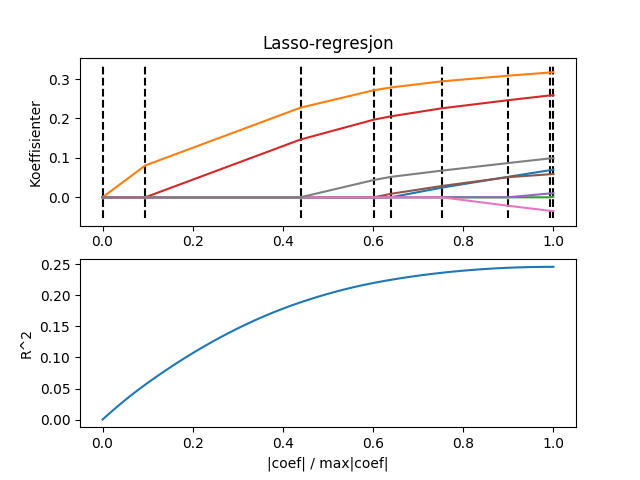
\includegraphics[height=0.8\textheight]{lasso.png}
  \end{center}
\end{frame}

\begin{frame}
  \frametitle{Prinsipalkomponent-regresjon}

  Matrisen \(\textbf{X}^T \textbf{X}\) kan dekomponeres (egenverdi-dekomposisjon):
  \begin{equation}
    \textbf{X}^T\textbf{X} = \textbf{VD}^2\textbf{V}^T
  \end{equation}

  der \(\textbf{V}\) er matrisen med egenvektorene til \(\textbf{X}^T\textbf{X}\) som kolonnevektorer og \(\textbf{D}^2\) er diagonalmatrisa med de korresponderende egenverdiene \(d_1^2 \geq d_2^2 \geq \dots \geq d_p^2\) som diagonalelementer.

  \pause

  Vi danner matrisa \(\textbf{Z} = \textbf{X}\textbf{V}\). Kolonnene i denne matrisa kalles \emph{prinsipalkomponentene} til \textbf{X}.

\end{frame}

\begin{frame}
  \frametitle{Prinsipalkomponent-regresjon}

  Prinsipalkomponent-regresjon utføres ved at man velger de \(k\) første prinsipalkomponentene til \(X\), dvs. de første \(k\) kolonnene til \(Z\) og gjør minste kvadrater på denne matrisa.
\end{frame}

\begin{frame}
  \frametitle{Prinsipalkomponent-regresjon}
  \begin{center}
    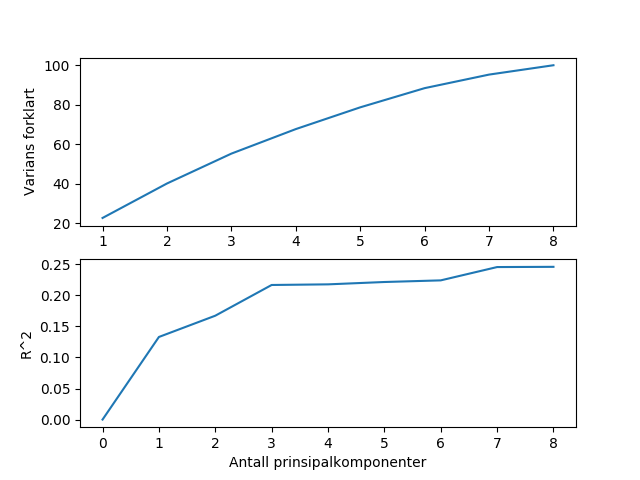
\includegraphics[height=0.8\textheight]{pcr.png}
  \end{center}
\end{frame}

\begin{frame}
  \frametitle{Parametervalg}
  Aller først delte jeg datasettet i to deler: Ett treningssett med 3108 (\(80\%\)) pasienter og et valideringssett med 777 (\(20\%\)) pasienter.
  \pause
  For å bestemme parameterene til de tre metodene, brukte jeg kryss-validering.
  \pause
  \begin{itemize}
    \pause
    \item Treningssettet ble delt inn i 10 grupper.
    \pause
    \item Hver modell og valg av parameter ble trent på 9 grupper og testet på den siste.
    \pause
    \item Dette ble gjentatt for hver gruppe.
    \pause
    \item Vi estimerte prediksjonserroren og standard-erroren til denne estimatoren.
    \pause
    \item Jeg bestemte parameteren ved å bruke \emph{én standard-error}-regelen.
  \end{itemize}
\end{frame}

\begin{frame}
  \frametitle{Beste delmengde-utvalg}
  \begin{center}
    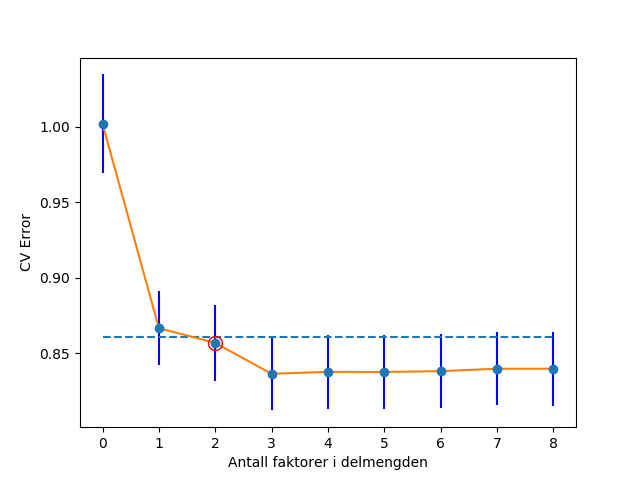
\includegraphics[height=0.8\textheight]{best_subset_CV.png}
  \end{center}
\end{frame}

\begin{frame}
  \frametitle{Lasso-regresjon}
  \begin{center}
    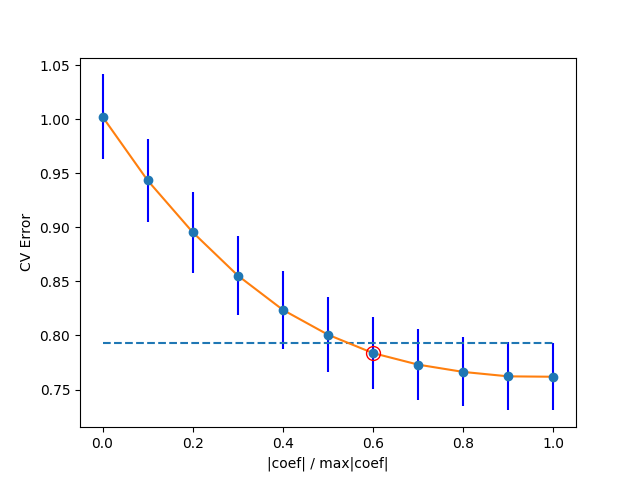
\includegraphics[height=0.8\textheight]{lasso_CV.png}
  \end{center}
\end{frame}

\begin{frame}
  \frametitle{Prinsipalkomponent-regresjon}
  \begin{center}
    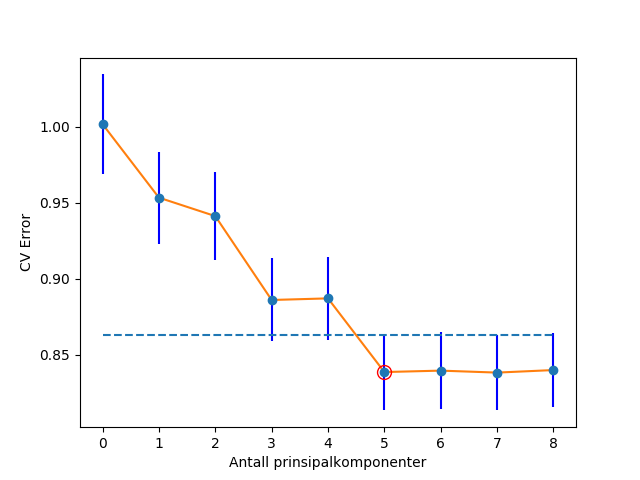
\includegraphics[height=0.8\textheight]{pcr_CV.png}
  \end{center}
\end{frame}

\begin{frame}
  \frametitle{Resultater}
  \begin{tabular}{ l r r r r}
    Prediktor & Minste kvadrater & Beste delmengde & Lasso & PCR \\
    \hline
    Kjønn & 0.070 & & & 0.008 \\
    Alder & 0.317 & 0.356 & 0.271 & 0.214 \\
    Sigaretter per dag & 0.002 & & & -0.080 \\
    BMI & 0.259 & 0.275 & 0.196 & 0.171 \\
    Diabetiker & 0.010 & & & 0.040 \\
    Glukose-nivå & 0.059 & & & 0.047 \\
    Utdanningsnivå & -0.034 & & & -0.148 \\
    Kolesterol-nivå & 0.099 & & 0.043 & 0.176 \\
    \hline
    Test Error & 0.723 & 0.720 & 0.733 & 0.776 \\
    Std Error & 0.039 & 0.039 & 0.040 & 0.041 \\
  \end{tabular}
\end{frame}

\begin{frame}
  \frametitle{Utvidelse av metodene}

  Jeg dannet nye prediktorer ved å ta alle mulige produkter av de originale: \[X_1 \cdot X_1, X_1 \cdot X_2, \dots.\]
  \pause
  Disse prediktorene ble brukt til å danne en ny matrise \(\textbf{X}\) bestående av både de originale og de nye prediktorene, tilsammen 44 prediktorer.
  \pause
  Jeg utførte så Lasso-regresjon og PCR på denne nye matrisen.
\end{frame}

\begin{frame}
  \frametitle{Lasso-regresjon (del 2)}
  \begin{center}
    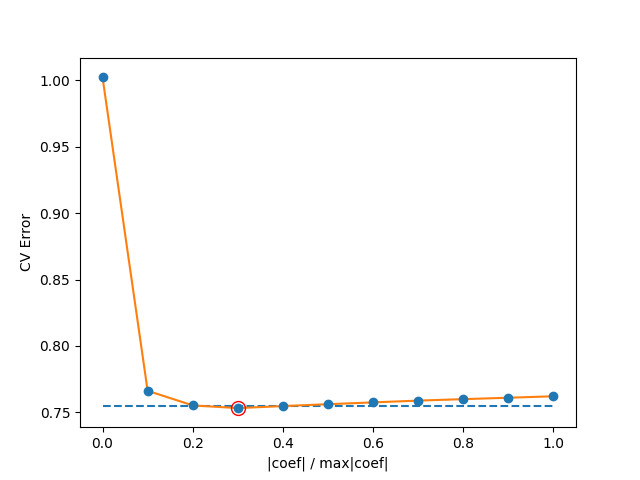
\includegraphics[height=0.8\textheight]{lasso_CV2.png}
  \end{center}
\end{frame}

\begin{frame}
    \frametitle{Prinsipalkomponent-regresjon (del 2)}
  \begin{center}
    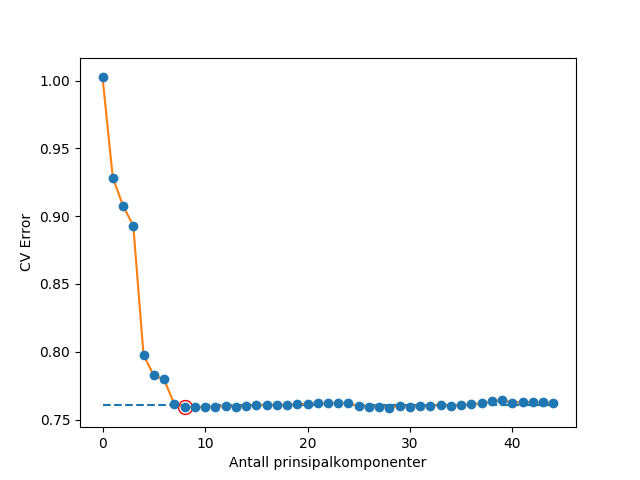
\includegraphics[height=0.8\textheight]{pcr_CV2.png}
  \end{center}
\end{frame}

\begin{frame}
  \frametitle{Resultater}
\begin{center}
  \begin{tabular}{ l r r}
     & Lasso & PCR \\
    \hline
    Test Error & 0.716 & 0.773 \\
    Std Error & 0.039 & 0.039
  \end{tabular}
  \end{center}
  Vi ser at test-erroren fra lasso-regresjonen ble forbedret fra 0.733 til 0.716.
\end{frame}

\end{document}
